\chapter{Introduction}\label{sec:intro}
With the explosive image resources people uploaded every day, image recognition becomes a very hot topic and has draw many attentions in recent years. Every year, there are many inspiring results in the ImageNet Large Scale Visual Recognition Challenge (ILSVRC). 
With development of recognition technology, many IT companies want to use image recognition techniques to serve their customers and many interesting applications have been developed, such as HowOld from Microsoft and Im2Calories from Google.

In order to successfully capture the diversity of different objects around us, many recognition models contain thousands or sometimes even millions of parameters and require large amount of training images to tune these parameters as well.
As the visual recognition system become increasingly successful in many general recognition tasks, people wish that it can solve the recognition problems in many new and complicated areas which are paid less attention before.
Unfortunately, for some real applications, it is often difficult and cost to collect large set of training images. Moreover, most algorithms require that the training examples should be aligned with a prototype, which is commonly done by hand. In many real applications, collecting and fully annotating these images can be extremely expensive and could have a significant impact on the over cost of the whole system. As a result, the challenge can come from these two aspects
\begin{enumerate}
	\item Abundant new categories/scenario. In some tasks, it is required for the system to learn new categories or scenarios. The recognition algorithm should be more dynamic to adapt the new categories and scenarios.
	\item Constraint on the training images. As these tasks are lack of attention before, the training data is rare. The annotation process of these data could be both expensive and time-consuming. 
\end{enumerate} 

On the other hand, recognition is one of the most important part of our human visual system. We can recognize various kinds of materials (apple, orange, grape), objects (vehicles, buildings) and natural scenes (forests, mountain). At the age of six, human can recognize about $10^4$ object categories\cite{biederman1987recognition}. 
Our human can learn and recognize a new object with just a glance, which means we can capture the diversity of forms and appearances of a objects with just a handful examples. This remarkable ability is obtained by effectively leveraging the learned knowledge and applying it to the new tasks. It could be ideal if there is a visual recognition model can have such ability, which is referred to as \textbf{Visual Transfer Learning} (VTL). 

VTL has been increasing popular with the success of modern image recognition algorithms. In VTL, the source domain is referred to the one we have already learned and the target domain is the one we actually want to learn. In VTL, measuring the relatedness of the source and target tasks is important for the transfer process.
In previous studies of VTL, people assume that the source data are always available and can be freely accessed. Therefore, the relatedness of the source and target domain can be effectively measured by comparing the data in two domains. However, this assumption is rarely hold in real applications. Source data are often a subject of legal, technical and contractual constraints between data owners and data customers. Beyond privacy and disclosure obligations, customers are often reluctant to share their data. When operating customer care, collected data may include information on recent technical problems which is a highly sensitive topic that companies are not willing to share.
On the other hand, sharing the model trained from the source data, i.e. the source model, instead of the data can avoid these obligations and is more common in real applications. VTL under this situation is usually called \textbf{Hypothesis Transfer Learning} (HTL) \cite{kuzborskij2013stability} and the source model is called hypothesis.

In this thesis, we investigate the VTL problem under the HTL setting. 3 methods are proposed under the HTL setting for different learning scenarios.

\section{Overview for Image Recognition}\label{sec:intro:over}
In this section, we review the major procedures for image recognition. 
A general image recognition method consists of three parts: image preprocess, feature extraction and classification.

\begin{figure}
	\centering
	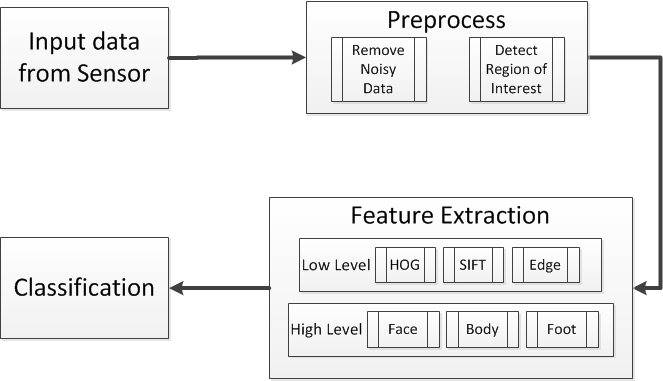
\includegraphics[scale=.8]{introduction/fig/IRflow.png}
	\caption{Major procedure for image recognition.}\label{fig:intro:irflow}
\end{figure}
\subsection{Preprocess}
Firstly, the optical property of an object is captured through its optical sensor of a digital camera and then the digital camera generates raw digital data of the image.
After receiving the raw data of a image from the sensor, preprocess is to generate a new image from the source image. This new image is similar to the source image, but differs from it considering certain apsects, e.g. the new image has smoother edge, better contrast and less noise. 
Here, some \textit{pixel operations} and \textit{local operations} are used to improve the contrast and remove the noise.  

Another important operation of preprecess is segmentation according to the object, i.e. finding the region of interest. Images used for recognition should be aligned, making the target object appear in the central of the image and remove those irrelevant area.

The result of preprocess has great impact on the final result of the recognition. Clear and noise free images can make the feature extraction more effective and significantly improve the final classification accuracy.

\subsection{Feature Extraction}
Feature extraction is used to extract the optical properties of an image and represent interesting parts of an image from the raw image data as a compact feature vector. The feature vector is then used for either training the classifier or recognition. Therefore, feature extraction is the most important part for image recognition. The quality of the features extracted from a image have great impact on the recognition result. There are two major streams for feature extraction: the hand engineered method and representation learning method.
\subsubsection{Hand Engineered Feature}
Hand engineered features are typically low level and local features.
Low level features are extracted according to some optical properties of an image. These features are low level / local features. There is a widely agreement that local features are an efficient tool for object representation due to their robustness with respect to occlusion and geometrical transformations \cite{van2006coloring}. Common low level hand engineered features include Histogram of Oriented Gradients (HOG) \cite{dalal2005histograms}, Scale Invariant Feature Transform (SIFT) \cite{lowe1999object}, Speeded Up Robust Features (SURF) \cite{bay2006surf}, Local Binary Patterns (LBP) \cite{ojala2002multiresolution}, and color histograms \cite{birchfield1998elliptical}. Feature descriptors obtain from these low level features refer to a pattern or distinct structure found in an image, such as a point, the edges, or some small image patches. They are usually associated with an image patch that differs from its immediate surroundings by texture, color, or intensity. What the feature actually represents does not matter. We know that it is distinct from its surroundings.
\begin{figure}[h]
	\centering
	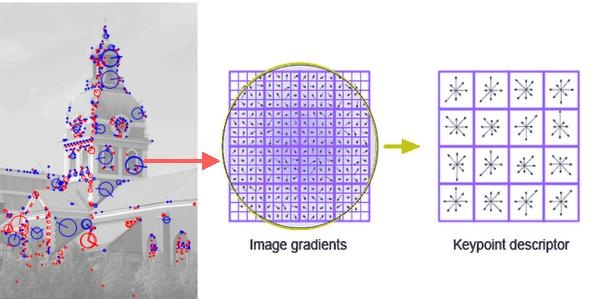
\includegraphics[scale=.6]{introduction/fig/sift.jpg}
	\caption{Feature extraction using SIFT.}\label{fig:intro:sift}
\end{figure}
These low level features can be used directly for recognition. However, since they just represent certain local properties of an image and are not discriminative enough for recognition, discriminative high level features can be further learned by combining the low level features using some algorithms such as bag-of-visual words\cite{lazebnik2006beyond}. 

\subsubsection{Representation Learning}
Representation learning is mainly described by Deep Learning 
algorithms\cite{krizhevsky2012imagenet} or Auto Encoders \cite{bengio2007scaling}. The ideas is to learn a group of filters that are able to capture various kinds of features to discern one category of images from the another category with some supervised or unsupervised algorithm. Typically in representation learning, features are learned hierarchically from low-level features to high level ones automatically. 
Learning representation from an image can start from either low level hand-crafted features (for Auto Encoders) or raw pixels of an image (for Deep Learning). 
\begin{figure}
	\centering
	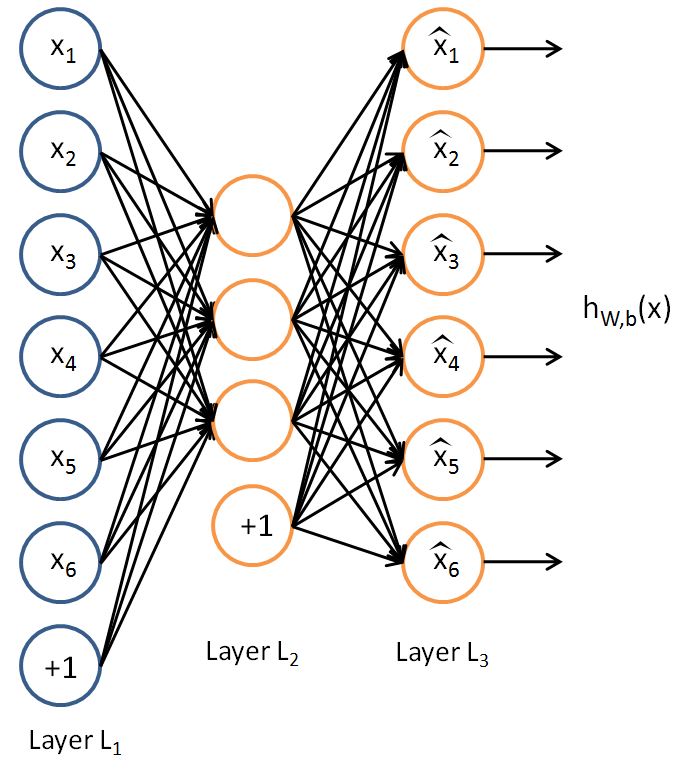
\includegraphics[scale=.3]{introduction/fig/sparsecoding.png}
	\caption{General Scheme of Auto Encoders. L1 is the input layer, possibly raw-pixel intensities. L2 is the compressed learned latent representation and L3 is the reconstruction of the given L1 layer from L2 layer. AutoEncoders tries to minimize the difference between L1 and L3 layers with some sparsity constraint.}\label{fig:intro:sparse}
\end{figure}

\textbf{Auto Encoders} are widely used to combine different types of low level feature. The outputs of the Auto Encoders are some latent representations. These latent representations are learned from the given images that have lowest possible reconstruction error. Even though the high level representations from Auto Encoders are learned by minimizing the reconstruction errors, they are still not robust enough to handle all kinds of variance of the objects in some tasks.

\textbf{Deep Learning} is the most popular approach for learning representations. It has been widely used for all kinds of image recognition tasks and achieved the state-of-the-art performance on some large scale image recognition tasks, such as ILSVRC and The PASCAL Visual Object Classes Challenge (PASCAL VOC). 
Convolutional Neural Networks (CNN) is the most popular deep learning model for the image recognition tasks\footnote{Deep CNNs are sometimes considered as the end-to-end classifier while learning the feature representation and discriminative classifier simultaneously. However, the feature representation learned from deep CNNs can still achieve good results with other classifiers and here we consider it as a feature extractor rather than a classifier.}. The first deep CNN that had great success on image recognition is the LeNet proposed by Y.LeCun in 1989 \cite{lecun1989backpropagation}. Backpropagation was applied to Convolutional Neural networks with adaptive connections. This combination, incorporating with Max-Pooling and speeding up on graphics cards has become an important part for  many modern, competition-winning, feedforward, visual Deep Learners. Deep CNNs have been widely used as the feature extractor for all kinds of images recognition tasks and proven to be the most powerful method of feature extraction.
\begin{figure}
	\centering
	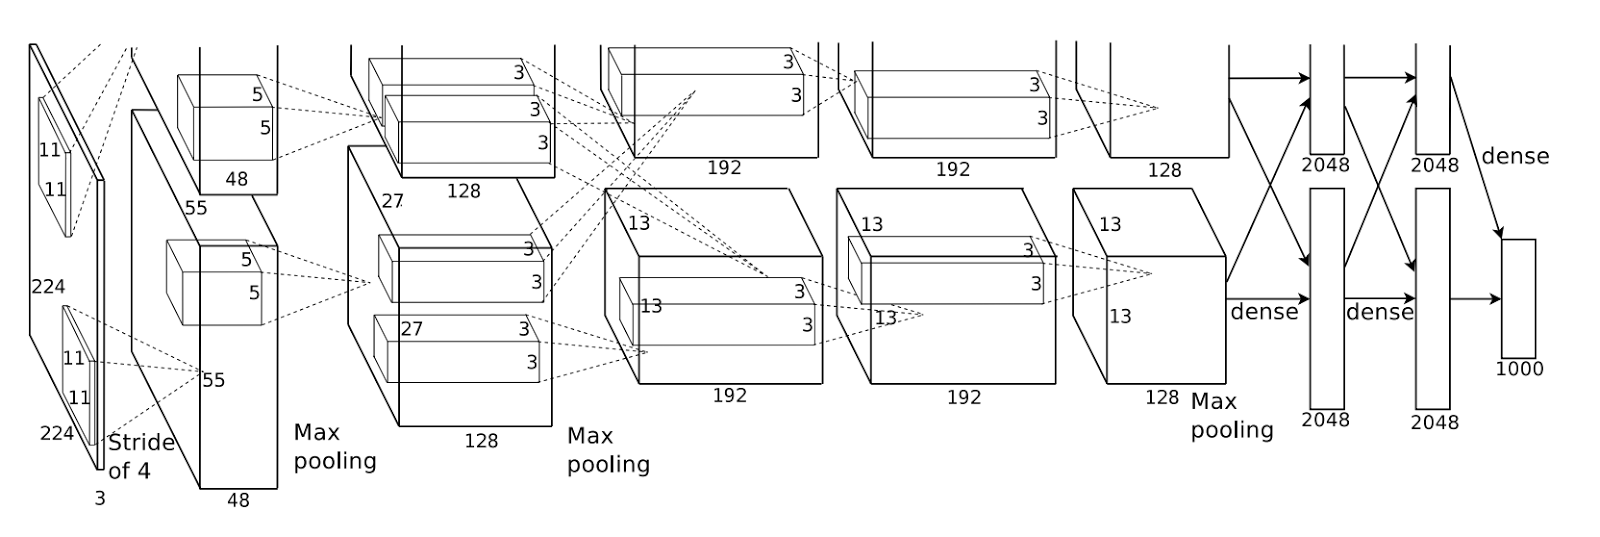
\includegraphics[scale=.3]{introduction/fig/alexnet.png}
	\caption{The architecture of ALEXNET (adopted from \cite{krizhevsky2012imagenet}).}\label{fig:intro:alex}
\end{figure}

\subsection{Classification}
After extracting feature representation from the images, a classifier is used to train a recognition model as well as for predicting the new coming images. A supervised model is always used for training the recognition model. Discriminative Classifier such as Support Vector Machine (SVM) is widely used as the classifier for recognition \cite{cristianini2000introduction}. As we mentioned before, in order to capture different variances of the images for one category, the size of the feature representation for an image is usually very large. In order to avoid overfitting, the size of the training set should be at least the same size of the feature representation as well. Some classifiers such as Bayesian method or decision tree require to consider the correlations between each feature and the class labels and suffer from the large feature dimension. However, Discriminative Models\cite{bottou2010large} are more convenient for training. Discriminative Models can be effectively optimized with stochastic gradient descent and are suitable for the large training set. 

However, to capture all variance of an object, training a good recognition model requires abundant data when we learn a model from scratch. With the limited training data, it is difficult to achieve a good classification performance. Transfer learning is an effective way to solve this problem by utilizing the knowledge from previous tasks. In this thesis, we focus on how to transfer the knowledge from the source domain for recognition tasks. The methods proposed in chapter \ref{sec:pakdd} and chapter \ref{sec:aaai} mainly focus on the stage of classification while the method in chapter \ref{sec:cnn} focuses on both feature representation learning and classification.




\section{Approaches in Visual Transfer Learning and the Limitations}
As we mentioned before, research of visual transfer learning focuses on designing classifiers that can leverage the source knowledge effectively. In this section, we briefly review methods for the visual transfer learning and show the limitation of previous work. 
\subsection{Intuition for Visual Transfer Learning}
The intuition of visual transfer learning comes from our human recognition mechanism. For our human, all the information acquired is stored in our memory. These information are organized according to the properties. When we see a new concept, we don't treat it isolated, but connect it to certain previous knowledge we stored in our memory. By comparing a new concept with the organized information in our memory, we can capture the property of a new concept effectively. When referring to visual tasks, several examples can be given to show this cognitive ability. For instance, when we describe the animal "okapi" (see Figure \ref{fig:intro:multi}), we would probably say that: okapi has a body of a horse, legs of the zebra and a head of giraffe. People who never see a zebra could instantly have a rough idea of a zebra. 

\begin{figure}
	\centering
	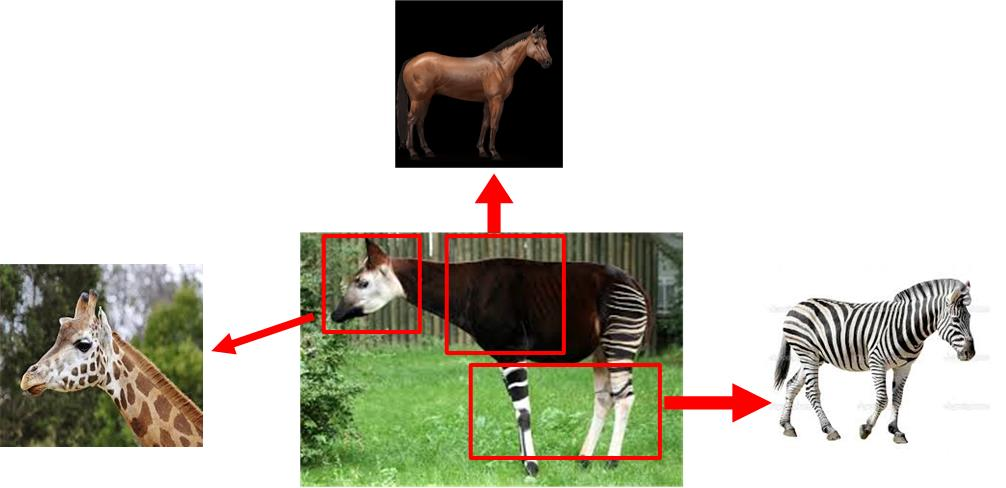
\includegraphics[scale=.6]{introduction/fig/multiple.jpg}
	\caption{An intuitive description for human to learn new concept: an okapi can be roughly described as the combination of a body of a horse, legs of the zebra and a head of giraffe.}\label{fig:intro:multi}
\end{figure}

This indicates that to learn a concept effectively, we should be able to make use of the gained knowledge instead of learn it from scratch. This process is commonly referred to as transfer learning\cite{pan2010survey}. Traditional machine learning methods work under the common assumption: training data and testing data are drawn from the same feature space and same distribution. 
In transfer learning, the test data can come from a different distribution. The data from the original distribution is called source data, and data from the new distribution is called target data. Transfer learning is used to utilize the source knowledge from the source data to help building the new model to classify the target data. 

\subsection{Approaches for Visual Transfer Learning}
Successfully leveraging the source knowledge can greatly improve the performance of the target model. In general, the more related the source and target domain are, the more useful the source knowledge is and the more benefit the target model can get. Leveraging unrelated knowledge cannot help to improve the performance of the target model or even hurt the it. Therefore, the key issue for visual transfer learning is to identify the relatedness of the source and target domain. The major approaches for Visual Transfer Learning consists of two main direction: Distribution Similarity Measurement and Instance Reuse.

\begin{itemize}
	\item \textbf{Distribution Similarity Measurement}. The core idea of transfer learning is to leverage the related source knowledge. The more related the source is, the better transfer performance we can achieve. Thus, measuring the the relatedness of the source knowledge is an important part in transfer learning especially where there are multiple sources. A straight-forward approach to identify the relatedness of the source and target domain is to measure their similarity directly. Measuring the data discrepancy through some statistical measurements such as \textbf{Maximum Mean Discrepancy} (MMD) \cite{duan2009domain}, has been a popular way to identify the source and target domain. MMD reflects the distance of two data distributions in the Reproducing Kernel Hilbert Space (RKHS) \cite{aronszajn1950theory}.
	\item \textbf{Instance Reuse}\cite{lim2012transfer}. Generally, we apply transfer learning under the scenario where the target data is scarce and we are not able to build the target model alone with the target data. A simple solution is to ``borrow" some of the data from the source domain and use it to build the target model together with the target data. This approach can directly increase the size of the data in the target domain and effectively improve the performance of the target model. For example, \textbf{Feature Transformation} \cite{duan2012learning} can overcome the data distribution mismatch in different domains and project the data into the same augmented space and thus can increase the training data for the target task as well (see Figure \ref{fig:intro:trans}).
\end{itemize}

\begin{figure}
	\centering
	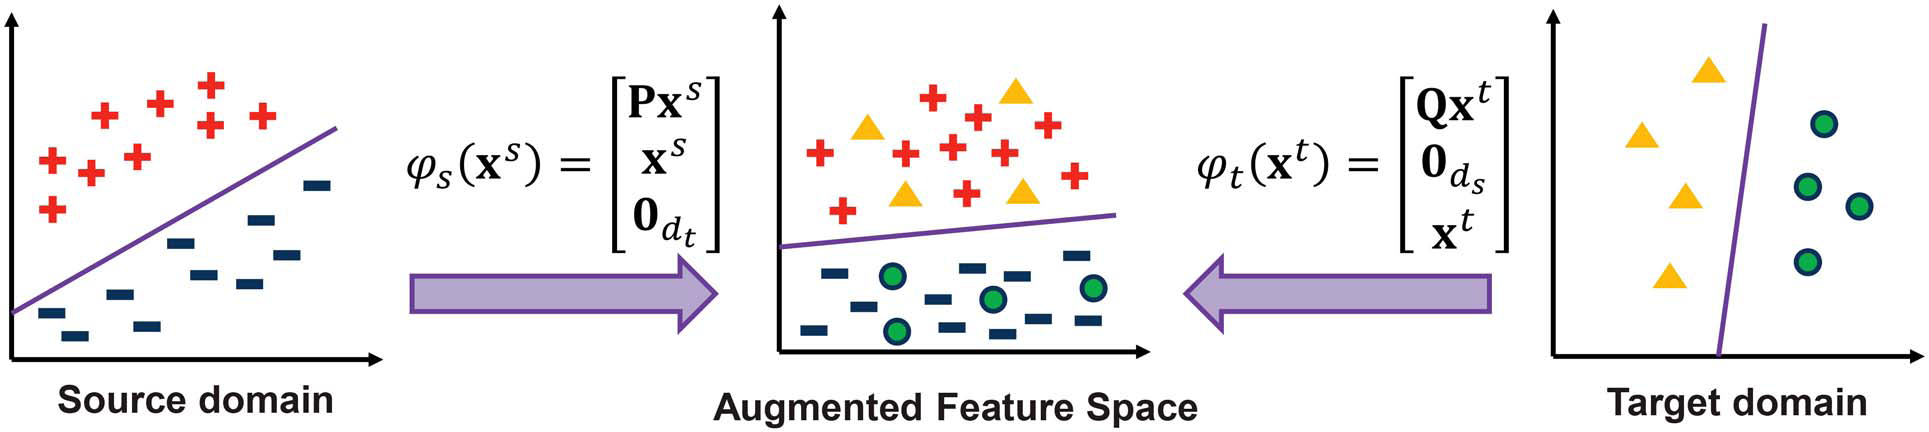
\includegraphics[scale=.3]{introduction/fig/transformation.png}
	\caption{Feature transformation. Transform the data in different domains into a augmented feature space.}\label{fig:intro:trans}
\end{figure}

\subsection{Limitation of Previous Methods}
From the review of the approaches for Visual Transfer Learning we can see that
most previous methods require access to the source data to obtain the source knowledge. However, in many practical problems, these previous approaches may not be as convenient as we thought due to the following reasons:

\begin{itemize}
	\item \textbf{Data accessibility}. The source data may not be able to access for some tasks. For example, clinical database is not allowed to access for general publics due to the privacy. Disclosure obligations and will to share the databases are also two important reasons that make the source data inaccessible.
	\item \textbf{Size of the source data}. Besides data accessibility, many previous methods \cite{daume2009frustratingly}\cite{duan2012learning} require to access to each of the individual source instance to obtain the source knowledge which is ineffective for many large source domain. For example, it is almost impossible to measure the MMD for some large source domain which contains hundreds of thousands instances.
\end{itemize}

From above we can see that these previous methods can successfully leverage the source knowledge under the assumption that the source data are freely accessible and relatively small. However, this assumption could fail in real applications. In some cases, the source data could be private (such as the clinic data from patients) and therefore, could not be shared with public. Moreover, those large source dataset generally contains more knowledge and information compared to the small ones and thus can better improve the transfer performance of the target task. However, obtaining the similarity measurement of these large dataset with those previous methods can be tedious and inefficient. It is important to find a way to leverage the source knowledge without accessing to the source data.

In this thesis, we assume that we can freely access to the source model trained from the source data and thus leverage the knowledge from the model instead. Using the source model for transfer learning can successfully avoid the two issues discussed above. Source model can contain as much knowledge as the source data while without containing any information regarding to the individual instance. Therefore, the owner of the source data does not have to worry about the leak of the privacy. For those large source dataset such as ILSVRC containing millions of images, a trained source model is normally a few megabytes and public available. Therefore, leveraging the source knowledge from source model instead of the source data itself is more practical for real visual transfer learning applications.
%%%%%%%%%%%%%%%%%%%%%%%%%%%%%%%%%%%%%%%%%%%%%%%%%%%%%%%%%%%%%%%%%%%%%%%%%%%%%%%%%

\section{Main Contribution}
In this section, we discuss the challenges that we may encounter when we can only access the source model. Then we demonstrate the learning scenarios and proposed solutions in this thesis.

\subsection{Challenges}
Despite for the general challenges in transfer learning, in our HTL settings, there are some new challenges in this thesis.

The first challenge is \textbf{knowledge representation}, i.e. how to obtain the source knowledge when we are not able to access to the source data. When source data is accessible, the source knowledge is relatively explicit and we can easily obtain the source knowledge by either analyzing the source data distribution or make use of the source data to help training the target mode. The knowledge of the source domain is implicit and encoded in the source model using certain learning algorithms. How to effectively extract the source knowledge from the models is challenging.

The second challenge is \textbf{knowledge expressiveness}, i.e. how to leverage the source knowledge to help training the target model. As the source knowledge is implicit, how to effectively leverage the source knowledge and improve the transfer performance is also important. We also expect that the source knowledge extracted from the source model should be as general as possible so that the source knowledge can be extracted from different types of source model. Therefore, our transfer learning algorithm can work in many situations. 

The last challenge is \textbf{knowledge regularization} i.e. how to guarantee the performance of our transfer method. 
Humans appear to have mechanisms for deciding when to transfer information, selecting appropriate sources of knowledge, and determining the appropriate level of abstraction \cite{torrey2009transfer}. 
A basic criterion for the knowledge transfer process is that leveraging the knowledge from the source model should not hurt the performance of the target model. Negative transfer \cite{pan2010survey} happens when the performance of target model degrades after receiving the knowledge from the source domain and how to avoid negative transfer is still an open question to all transfer learning researchers. The absence of the source data makes the situation more complicated.

\subsection{Two Transfer Learning Scenarios}
In this thesis, we mainly focus on two transfer learning scenarios: inductive transfer learning for new classes and domain adaptation. The definition of the two scenarios is as follows:
\begin{definition}{\textbf{Domain Adaptation}}
	Let $X$ be the input space and $Y$ be output space. Given the source domain $D_s$ and the target learning task $D_t$ with marginal distribution $P(X_s)$ and $P(X_t)$, we assume that $D_s$ and $D_t$ share the same conditional distribution $P(Y|X)$. The goal of Domain Adaptation is to learn the $P(X_t|Y_t)$ for the target task with the help of $D_s$.
\end{definition}

\begin{definition}{\textbf{Inductive Transfer Learning}}\cite{pan2010survey}
	Given a source domain $D_s$ and the source learning task $T_s$, a target domian $D_s$ and the target learning task $D_t$, inductive transfer learning aims to help improve the learning of the target task function $f_t(\cdot)$ in $D_t$ using the knowledge from $D_s$ and $D_s$ where $D_s \neq D_t$.
\end{definition}

The major difference between the two transfer learning scenarios is that in inductive transfer learning, the source and target tasks are two different but related tasks (e.g. from sport car to heavy truck) while in domain adaptation, the source and target tasks are the same task but with different marginal distributions (e.g. from the animation dog to the real dog). 

\begin{figure}[h]
	\centering
	\subfloat[Domain Adaptation]{\includegraphics[scale=.4]{introduction/fig/da.png}}
	\qquad
	\subfloat[Inductive transfer learning the new class]{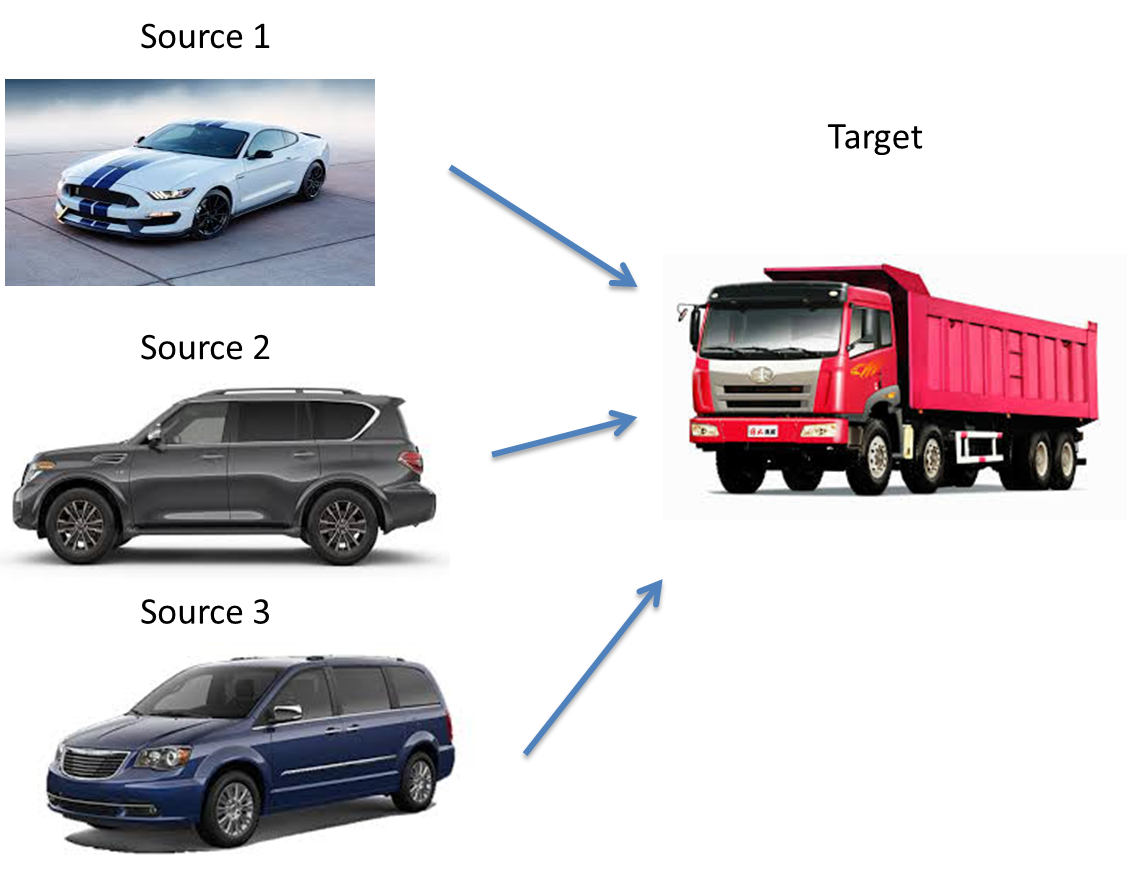
\includegraphics[scale=.33]{introduction/fig/ind.png}}
	\caption{Difference between two transfer learning scenarios}\label{fig:intro:cmp}
\end{figure}


\subsection{Proposed Methods}
There are three methods proposed in this thesis, one in inductive transfer learning for new classes and two methods in domain adaptation.


In chapter \ref{sec:pakdd}, we extend the previous methods in HTL which are limited to using SVMs as the source model and propose a novel method \textbf{Effective Multi-class Transfer Learning} (EMTLe) for supervised domain adaptation. We use the output of the source model as the auxiliary bias to adjust the target model. Here, the output of the source model is used as the prior to adjust the decision for the target model. As long as we can set a proper weight to the prior knowledge, the source model can serve well for the target task. Because we only require the source model to provide its decision, we can treat it as a black-box model and EMTLe can leverage the source model from any source classifier that can generate the class probability of an example.

In chapter \ref{sec:aaai}, we investigate the problem of semi-supervised domain adaptation where most of the data in the target task are unlabeled and propose a novel framework \textbf{Generalized Distillation Semi-supervised Domain Adaptation} (GDSDA). In GDSDA, the source model generates ``soft labels" for the target data and can improve the performance together with the true labels from target task. Arguably, we use the imitation parameter to determine the relative importance of the soft label and true label. Then we propose GDSDA-SVM that can determine the imitation parameter autonomously through cross-validation.

In chapter \ref{sec:cnn}, we use the deep neural network to solve the transfer learning problem for food recognition. We use GoogLeNet trained from ImageNet of 1000 classes as our source model and two food databases as our target task, containing 101 classes and 265 classes respectively. In this chapter, we don't treat the source model as a black-box. Instead, we can obtain the parameters of the original GoogLeNet. We re-use the parameters in the original GoogLeNet as the prior and fine-tune it on our target task to achieve the improved performance. By re-using and fine-tuning the parameter, i.e. features from source tasks, we can effectively learn new categories of the target task. We show that without accessing the source data, we can still achieve better performance compared to previous methods.
\section{Summary}
In this chapter, we briefly introduced the problems that are solved in this thesis. We first demonstrate the procedure for image recognition and introduce some previous work for visual transfer learning. Then we pointed out the limitations of the previous work and proposed our methods under two transfer scenarios.